\documentclass[12pt,]{article}
\usepackage{lmodern}
\usepackage{amssymb,amsmath}
\usepackage{ifxetex,ifluatex}
\usepackage{fixltx2e} % provides \textsubscript
\ifnum 0\ifxetex 1\fi\ifluatex 1\fi=0 % if pdftex
  \usepackage[T1]{fontenc}
  \usepackage[utf8]{inputenc}
\else % if luatex or xelatex
  \ifxetex
    \usepackage{mathspec}
  \else
    \usepackage{fontspec}
  \fi
  \defaultfontfeatures{Ligatures=TeX,Scale=MatchLowercase}
\fi
% use upquote if available, for straight quotes in verbatim environments
\IfFileExists{upquote.sty}{\usepackage{upquote}}{}
% use microtype if available
\IfFileExists{microtype.sty}{%
\usepackage{microtype}
\UseMicrotypeSet[protrusion]{basicmath} % disable protrusion for tt fonts
}{}
\usepackage[margin=0.50in]{geometry}
\usepackage{hyperref}
\hypersetup{unicode=true,
            pdftitle={Analysis of integration site distributions and clonal abundances for gene therapy correction of cystinosis},
            pdfauthor={John K. Everett, Ph.D.~and Frederic Bushman, Ph.D.},
            pdfborder={0 0 0},
            breaklinks=true}
\urlstyle{same}  % don't use monospace font for urls
\usepackage{graphicx,grffile}
\makeatletter
\def\maxwidth{\ifdim\Gin@nat@width>\linewidth\linewidth\else\Gin@nat@width\fi}
\def\maxheight{\ifdim\Gin@nat@height>\textheight\textheight\else\Gin@nat@height\fi}
\makeatother
% Scale images if necessary, so that they will not overflow the page
% margins by default, and it is still possible to overwrite the defaults
% using explicit options in \includegraphics[width, height, ...]{}
\setkeys{Gin}{width=\maxwidth,height=\maxheight,keepaspectratio}
\IfFileExists{parskip.sty}{%
\usepackage{parskip}
}{% else
\setlength{\parindent}{0pt}
\setlength{\parskip}{6pt plus 2pt minus 1pt}
}
\setlength{\emergencystretch}{3em}  % prevent overfull lines
\providecommand{\tightlist}{%
  \setlength{\itemsep}{0pt}\setlength{\parskip}{0pt}}
\setcounter{secnumdepth}{0}

%%% Use protect on footnotes to avoid problems with footnotes in titles
\let\rmarkdownfootnote\footnote%
\def\footnote{\protect\rmarkdownfootnote}

%%% Change title format to be more compact
\usepackage{titling}

% Create subtitle command for use in maketitle
\newcommand{\subtitle}[1]{
  \posttitle{
    \begin{center}\large#1\end{center}
    }
}

\setlength{\droptitle}{-2em}
  \title{Analysis of integration site distributions and clonal abundances for
gene therapy correction of cystinosis}
  \pretitle{\vspace{\droptitle}\centering\huge}
  \posttitle{\par}
  \author{John K. Everett, Ph.D.~and Frederic Bushman, Ph.D.}
  \preauthor{\centering\large\emph}
  \postauthor{\par}
  \predate{\centering\large\emph}
  \postdate{\par}
  \date{April 2018}

\usepackage{booktabs}
\usepackage{longtable}
\usepackage{array}
\usepackage{multirow}
\usepackage[table]{xcolor}
\usepackage{wrapfig}
\usepackage{float}
\usepackage{colortbl}
\usepackage{pdflscape}
\usepackage{tabu}
\usepackage{threeparttable}
\usepackage[normalem]{ulem}

\usepackage{caption}

\begin{document}
\maketitle

{
\setcounter{tocdepth}{2}
\tableofcontents
}
\captionsetup[table]{labelformat=empty}

\newpage

\section{Summary of results}\label{summary-of-results}

The goal of this analysis is to investigate the integration profile of a
gene therapy vector for the correction of cystinosis in both mouse and
human subjects and assess potential clonal expansions. The list of human
oncogenes used throughout this analysis was compiled from the literature
(\href{http://www.bushmanlab.org/assets/doc/allOnco_Feb2017.tsv}{link})
and the list of mouse oncogenes was compiled from the retroviral tagged
cancer gene database (RTCGD)\textsuperscript{1} using an inclusion
threshold of three or more incidents. The human oncogene list comprises
7.46\% of all human genes (NCBI RefSeq) whereas the mouse oncogene list
comprises 2.01\% of all mouse genes. The frequency of integration sites
in human subjects near oncogenes was not significantly different than a
published trial using a comparable vector to correct Wiskott-Aldrich
syndrome (WAS) from which no adverse events have been
reported\textsuperscript{2}. The frequency of integration sites in bone
marrow donor mice near oncogenes was generally less than that of mice in
a previously published \(\beta\)-thalassemia mouse trial from which no
adverse events have been reported \textsuperscript{3}. The integration
position profile for human subjects was very similar to that found in
the WAS trial. The mouse bone marrow transplant trials yielded varying
degrees of persistence in five of the nine trials where detection was
limited due to both sequencing depth and vector copy number. No
significant enrichment of integration events near oncogenes was
identified between donor and recipient mice. The code base for this
analysis is available on-line
(\href{https://github.com/everettJK/project.geneTherapy.ucsdMouseCystinosis}{link}).

\vspace{0.1cm}

\section{Human and mouse samples
studied}\label{human-and-mouse-samples-studied}

Integration sites were detected in 74 samples from both human and mouse
subjects (Tables 1 \& S1) while no integration sites were detected in 10
of the provided samples (Table S2).

\vspace{0.1cm}

\begin{table}[!h]

\caption{\label{tab:unnamed-chunk-2}Table 1. Overview of data collection.}
\centering
\begin{tabular}[t]{lrlll}
\toprule
organism & samples & nReads & nFrags & nSites\\
\midrule
human & 30 & 19,834,249 & 132,619 & 93,050\\
mouse & 44 & 22,064,342 & 91,576 & 5,346\\
\bottomrule
\end{tabular}
\end{table}

\vspace{0.1cm}

\section{UCSC browser exploration}\label{ucsc-browser-exploration}

UCSC browser sessions pre-loaded with the integration sites identified
in this analysis are available via these links:
(\href{http://genome.ucsc.edu/cgi-bin/hgTracks?org=human\&db=hg38\&hgt.customText=http://microb120.med.upenn.edu/UCSC/cherqui/UCSC_CYS_human.ucsc}{human
subjects}),
(\href{http://genome.ucsc.edu/cgi-bin/hgTracks?org=mouse\&db=mm9\&hgt.customText=http://microb120.med.upenn.edu/UCSC/cherqui/UCSC_CYS_mouse.ucsc}{mouse
subjects}). You may have to allow your browser to open a new browser
window. Integration sites are shown as blue (positive orientation
integration) and red (reverse orientation integration) tick marks. For
each integration site, a second track provides the maximum clonal
abundance. Entering gene names into the search bar will direct the
browser to specific genes.

\newpage

\section{Description of analysis
techniques}\label{description-of-analysis-techniques}

We investigate effects of integration on cell growth using the following
criteria: Integration Frequency is the frequency at which unique
integration sites are observed in or near a given gene. Clonal Abundance
is determined by quantifying the number of sites of linker ligation
associated with each unique integration site. This samples the number of
DNA chains at the start of the experiment allowing clonal expansion to
be quantified\textsuperscript{4}.

Relative clonal Abundance is determined per sample and is the percentage
of identified cells attributed to a given clone. Integration sites and
the clones harboring them are sampled from a larger population. It would
be rare for all integration sites in a sample to be represented in the
sequence data.

For this analysis, four technical replicates of each delivered sample
were prepared, sequenced and analyzed with the INSPIIRED integration
site analysis pipeline (v1.2)\textsuperscript{5}.

\newpage

\section{Comparisons to previous
trials}\label{comparisons-to-previous-trials}

\subsection{Integration events near oncogenes in human
subjects}\label{integration-events-near-oncogenes-in-human-subjects}

In order to determine if the experimental vector has a higher propensity
of integrating near suspected oncogene in humans than previously
employed vectors, the frequency of integration near oncogenes was
compared to a previously published human trial\textsuperscript{1} which
used a comparable lentiviral vector to correct Wiskott-Aldrich syndrome
(WAS) where no adverse events have been reported to date. The frequency
of integration near oncogenes in four WAS pre-transplant patient samples
was compared to the frequency of integration in the experimental day 14
samples (Figure 1 {[}CYS: gray, WAS: blue{]}). The frequencies of
integration near oncogenes of samples in this study and the previous WAS
study were not significantly different (Mann-Whitney U-test p-value:
0.798).

\vspace{0.1cm}

\emph{Figure 1. Comparison of frequencies of integration events near
oncogenes.}\\
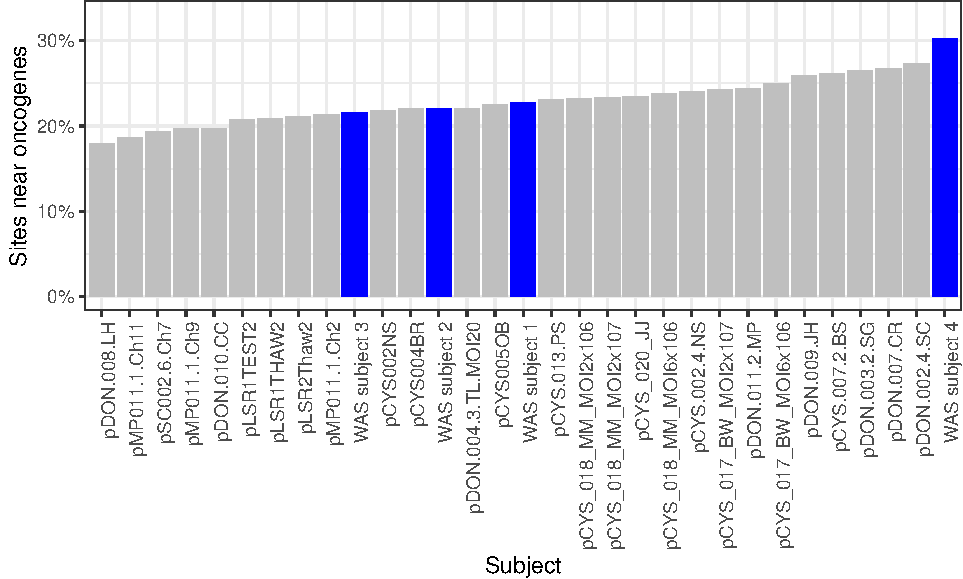
\includegraphics{project_files/figure-latex/fig1-1.pdf}

\newpage

\subsection{Integration events near oncogenes in mouse
subjects}\label{integration-events-near-oncogenes-in-mouse-subjects}

\vspace{0.1cm}

In order to determine if the experimental vector has a higher propensity
of integrating near suspected oncogene in mice than previously employed
vectors, the frequency of integration near oncogenes was compared to a
previously published mouse trial\textsuperscript{3} which used a
comparable lentiviral vector to correct \(\beta\)-thalassemia. The
frequency of integration events near onco genes in bone marrow donor
mice was generally less than the mean frequency of integration events
near oncogenes in the published trial (Figure 2 {[}CYS: gray,
\(\beta\)-thalassemia trial: blue{]}).

\emph{Figure 2. Comparison of frequencies of integration events near
oncogenes.}

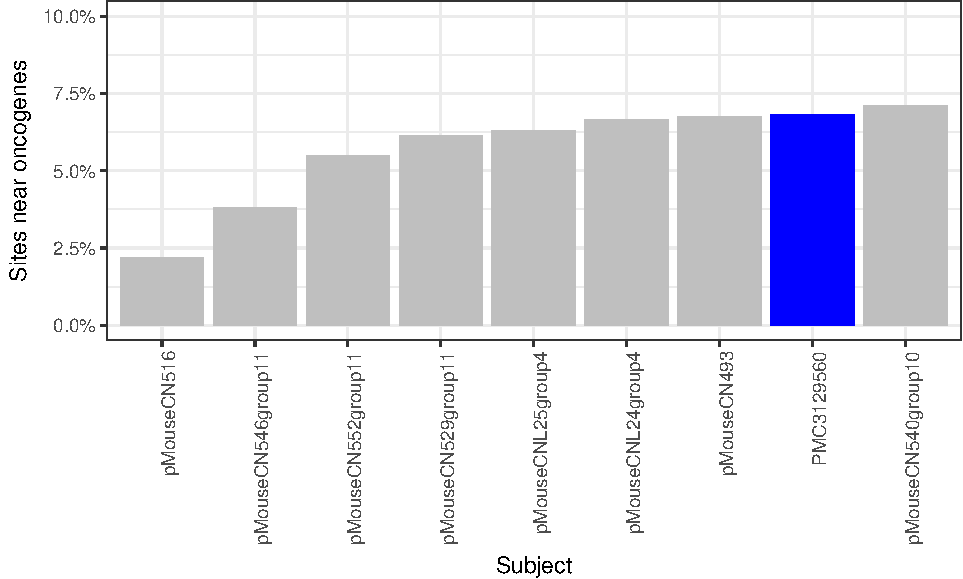
\includegraphics{project_files/figure-latex/fig2-1.pdf}

\newpage

\section{Mapping of integration site
positions}\label{mapping-of-integration-site-positions}

Heat maps of identified integration sites are shown below in Figure 3a
(human subjects) \& 3b (mouse subjects). The integration position
profile from human subjects is very similar to the profile from the
previous WAS study (Figure S2).

\emph{Figure 3a}

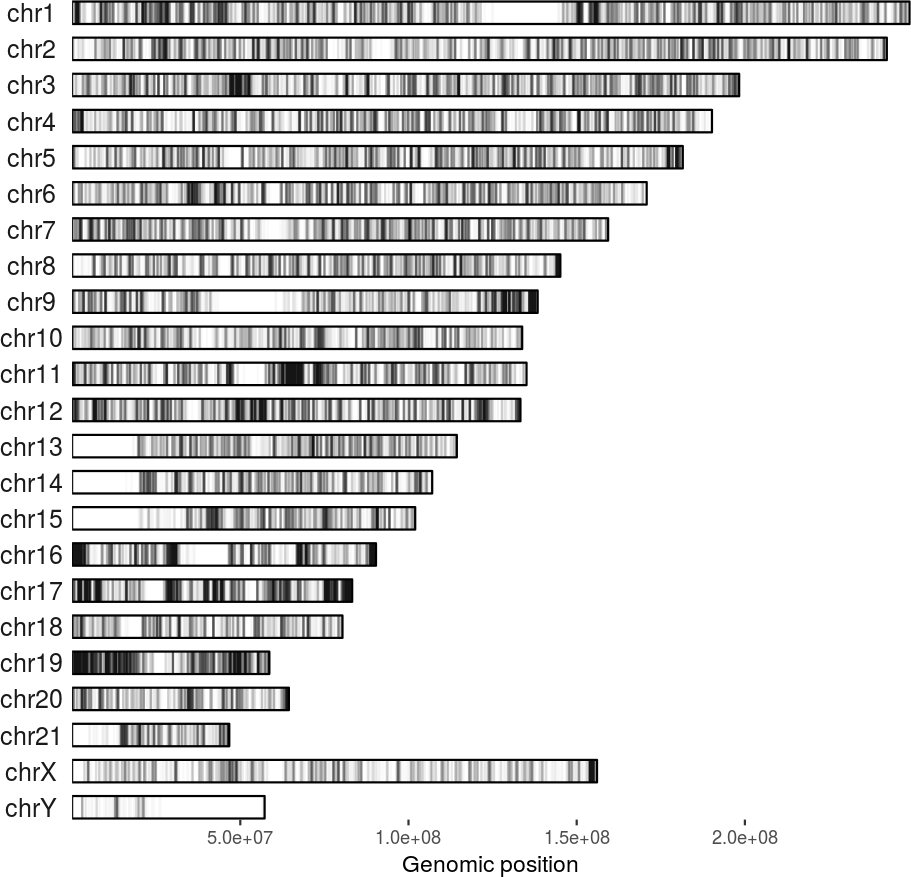
\includegraphics{project_files/figure-latex/fig3a-1.png}

\newpage

\emph{Figure 3b.}

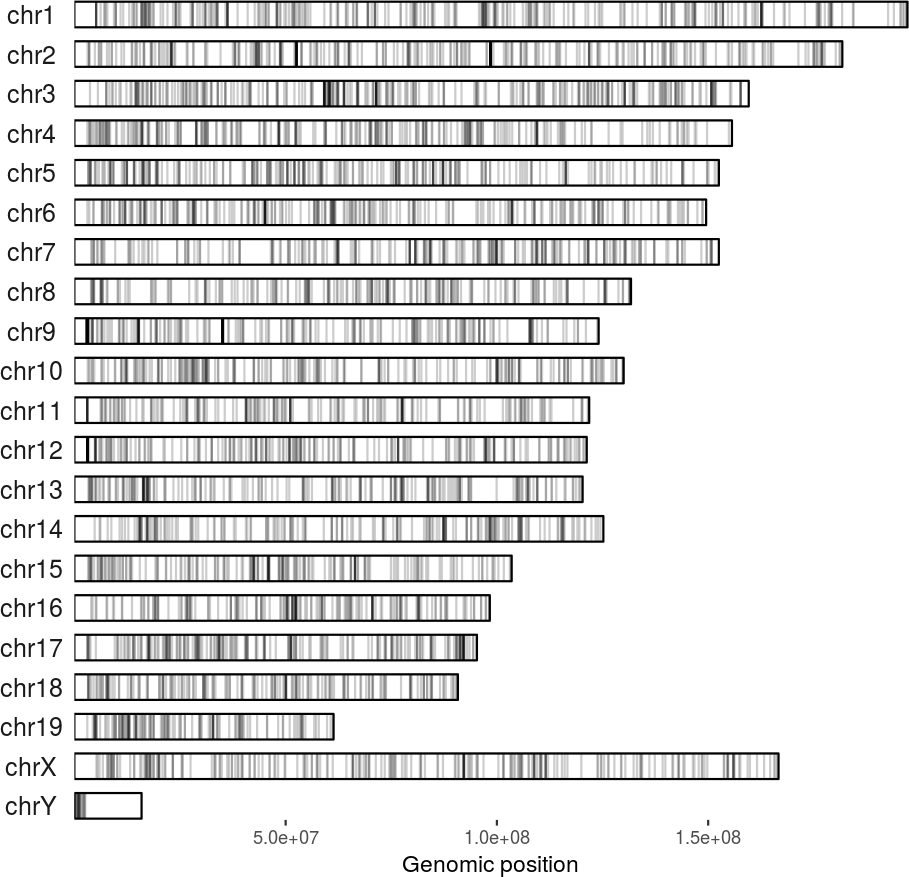
\includegraphics{project_files/figure-latex/fig3b-1.png}

\newpage

\section{Relative abundances of human subject
samples}\label{relative-abundances-of-human-subject-samples}

The sample relative abundance plots below (Figure 4) show the most
abundant 25 clones in each human sample as colored bars while less
abundant clones were relegated to a single low abundance bar shown in
gray. Subject DON.002.4.SC showed an expanded clone (30\% relative
abundance) with an integration event down stream of the non-coding RNA
LOC105374704. Subject DON.007.CR showed an expanded clone (15\% relative
abundance) with three integration events within ZNF337. These two
expanded clones are not of immediate concern given that such expanded
clones appeared in the WAS trial used for comparison (Figure S1) and
both samples contained relatively few inferred cells which inflate
relative abundance values.

\emph{Figure 4.}

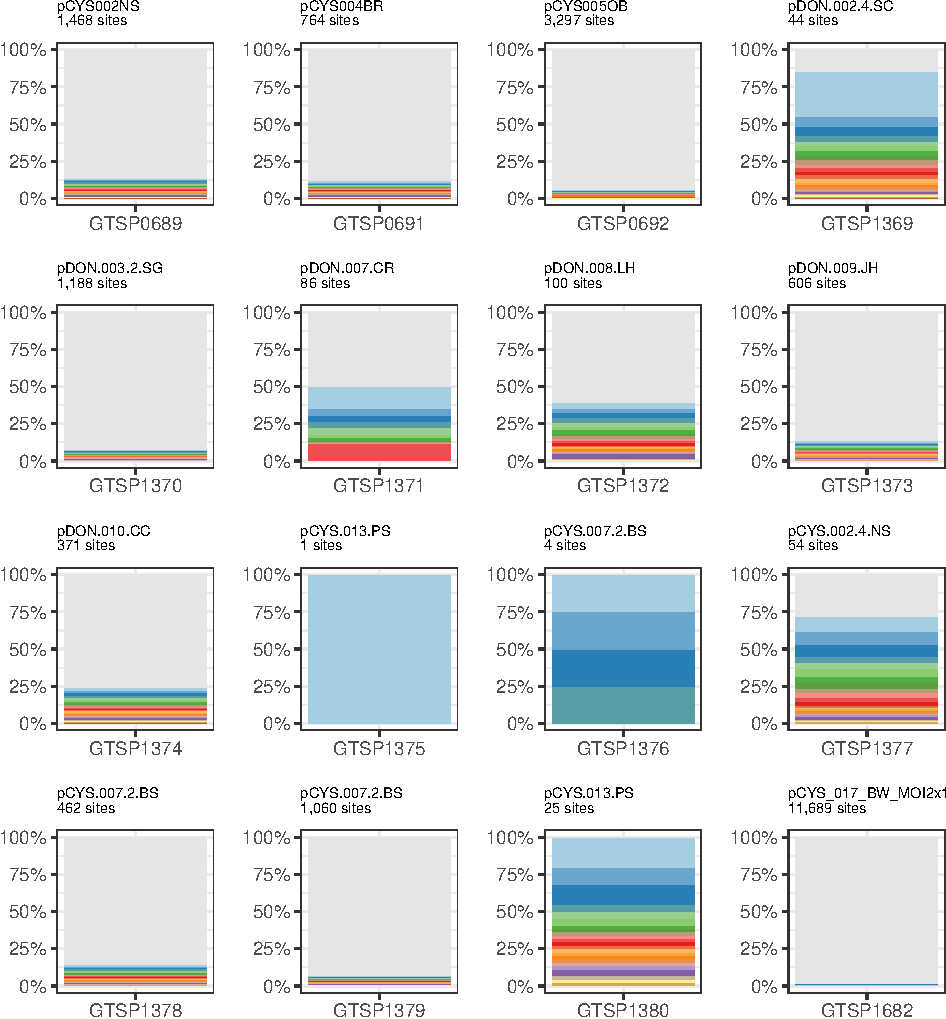
\includegraphics{project_files/figure-latex/fig4-1.pdf}

\newpage

\emph{Figure 4. (continued)}

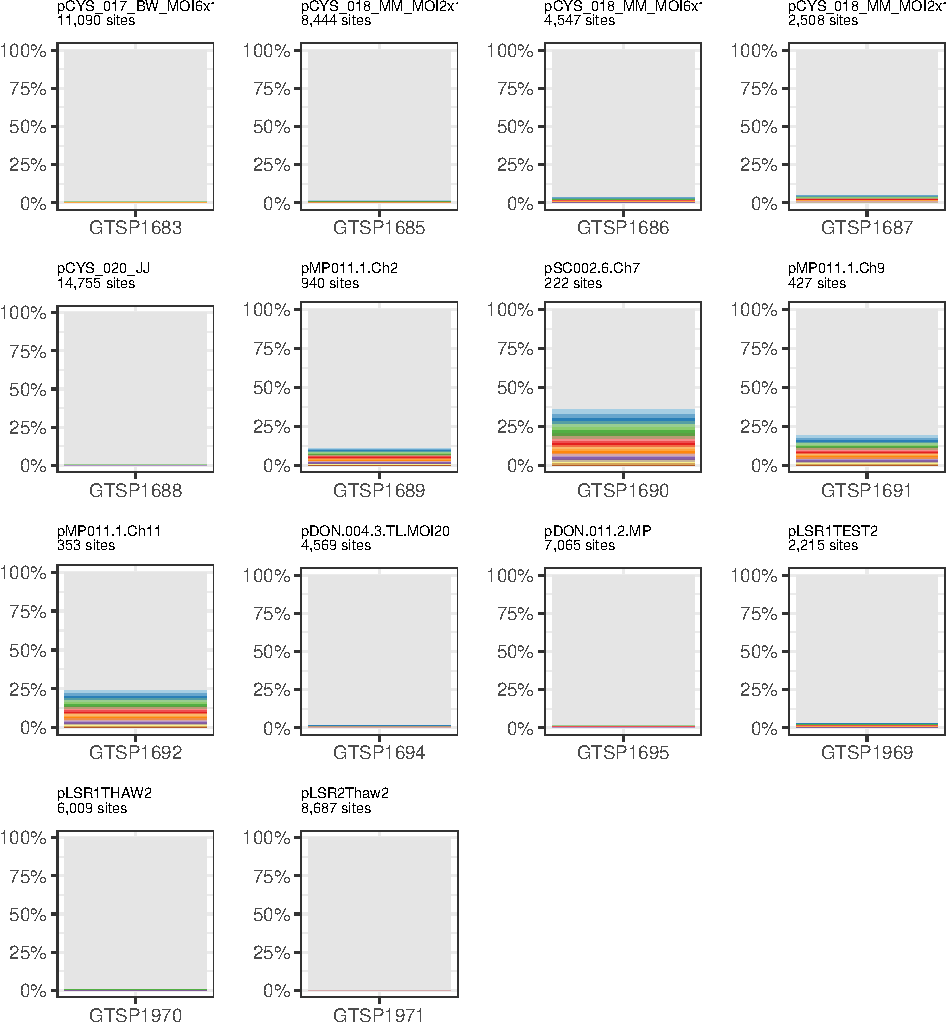
\includegraphics{project_files/figure-latex/fig4cont-1.pdf}

\newpage

\section{Expanded clones}\label{expanded-clones}

Table 2 below lists integration sites with relatives cell abundances
\(\geq\) 20\%. These integration events may be driving cell division and
follow-up longitudinal studies may be warranted. The estimated number of
cells harboring each integration (estAbund) is shown for context.

\emph{Table 2.}

\begin{table}[H]
\centering\rowcolors{2}{gray!6}{white}

\resizebox{\linewidth}{!}{\begin{tabular}{llllllrl}
\hiderowcolors
\toprule
patient & organism & timePoint & cellType & posid & relAbund & estAbund & nearestFeature\\
\midrule
\showrowcolors
pDON.002.4.SC & human & D14 & PB\_CD34 & chr5+30409434 & 29.92\% & 38 & LOC105374704\\
pCYS.007.2.BS & human & D14 & PBCD34-mock & chr1-218477558 & 25.00\% & 1 & TGFB2\\
pCYS.007.2.BS & human & D14 & PBCD34-mock & chr1-167962238 & 25.00\% & 1 & DCAF6\\
pCYS.007.2.BS & human & D14 & PBCD34-mock & chr6+11842138 & 25.00\% & 1 & ADTRP\\
pCYS.007.2.BS & human & D14 & PBCD34-mock & chr8+133682373 & 25.00\% & 1 & LOC105375773\\
pCYS.013.PS & human & D14 & PBCD34-mock & chr12+82136325 & 100.00\% & 1 & LOC101928449\\
pCYS.013.PS & human & D14 & PBCD34-MOI40 & chr8+67244348 & 20.45\% & 9 & ARFGEF1\\
pMouseCNL24group4 & mouse & M6 & Mouse\_BM & chr2+141127890 & 37.44\% & 1796 & Macrod2\\
pMouseCNL23group4control & mouse & M6 & Mouse\_BM & chr3-59165408 & 33.33\% & 2 & Igsf10\\
pMouseCNL25group4 & mouse & M6 & Mouse\_BM & chr3-59165408 & 32.30\% & 2907 & Igsf10\\
pMouseCNL25group4 & mouse & M6 & Mouse\_BM & chr3+71430357 & 21.19\% & 1907 & Gm6634\\
pMouseCNL25group4 & mouse & M6 & Mouse\_BM & chr9+15188460 & 20.42\% & 1838 & Cep295\\
pMouseCNL24group4 & mouse & M6 & Mouse\_BM & chr18-79750998 & 25.58\% & 1227 & Setbp1\\
pMouseCNL24group4 & mouse & M6 & Mouse\_BM & chrX+48224394 & 24.70\% & 1185 & Stk26\\
pMouseCNL38group1A & mouse & M6 & Mouse\_BM & chr7-115316991 & 50.00\% & 1 & Olfr486\\
pMouseCNL38group1A & mouse & M6 & Mouse\_BM & chr14-102130900 & 50.00\% & 1 & Lmo7\\
pMouseCN493 & mouse & M6 & Mouse\_BM & chr14+15556797 & 21.72\% & 1769 & Slc4a7\\
pMouseCNL59 & mouse & M6 & Mouse\_BM & chr2+52586806 & 25.16\% & 525 & Stam2\\
pMouseCNL58 & mouse & M6 & Mouse\_BM & chr2+141127890 & 100.00\% & 3 & Macrod2\\
pMouseCNL59 & mouse & M6 & Mouse\_BM & chr3-59165408 & 33.06\% & 690 & Igsf10\\
pMouseCN493 & mouse & M6 & Mouse\_BM & chr6-10697710 & 26.54\% & 2161 & AA545190\\
pMouseCNL53 & mouse & M6 & Mouse\_BM & chr19+18123881 & 100.00\% & 1 & Pcsk5\\
pMouseCN493 & mouse & M6 & Mouse\_BM & chrX-111592392 & 29.17\% & 2375 & Klhl4\\
pMouseCN545group11 & mouse & M6 & Mouse\_BM & chr5-12432693 & 39.48\% & 2080 & Sema3d\\
pMouseCN545group11 & mouse & M6 & Mouse\_BM & chr18-15129653 & 44.06\% & 2321 & Kctd1\\
pCNL80 & mouse & M6 & Mouse\_BM & chr3+123970190 & 32.46\% & 37 & Tram1l1\\
pCNL82 & mouse & M6 & Mouse\_BM & chr10-40246905 & 50.00\% & 1 & Slc22a16\\
pCNL82 & mouse & M6 & Mouse\_BM & chr10+94767778 & 50.00\% & 1 & Cradd\\
pCNL59 & mouse & M6 & Bone Marrow & chr2+52586806 & 37.50\% & 33 & Stam2\\
pCNL59 & mouse & M6 & Bone Marrow & chr2+52586806 & 26.47\% & 18 & Stam2\\
pCNL59 & mouse & M6 & B Cells & chr2+52586806 & 38.89\% & 7 & Stam2\\
pCNL59 & mouse & M6 & Bone Marrow & chr3-59165408 & 25.00\% & 22 & Igsf10\\
pCNL59 & mouse & M6 & Bone Marrow & chr3-59165408 & 30.88\% & 21 & Igsf10\\
pCNL59 & mouse & M6 & B Cells & chr3+71430357 & 27.78\% & 5 & Gm6634\\
pCNL59 & mouse & M6 & Bone Marrow & chr9+15188460 & 23.86\% & 21 & Cep295\\
pCNL59 & mouse & M6 & Bone Marrow & chr9+15188460 & 29.41\% & 20 & Cep295\\
pCNL59 & mouse & M6 & B Cells & chr9+15188460 & 27.78\% & 5 & Cep295\\
pCN760 & mouse & 6M & Bone Marrow & chr1-99613407 & 25.00\% & 4 & Ppip5k2\\
pCN774 & mouse & 6M & Bone Marrow & chr1-21011655 & 20.09\% & 90 & Tram2\\
pCN803 & mouse & 6M & Bone Marrow & chr3+60155698 & 25.07\% & 565 & Mbnl1\\
pCN803 & mouse & 6M & Bone Marrow & chr14-105778668 & 24.76\% & 558 & 5430440P10Rik\\
\bottomrule
\end{tabular}}
\rowcolors{2}{white}{white}
\end{table}

\newpage

\section{Mouse transplant trials}\label{mouse-transplant-trials}

The positions of identified integration sites from cell transplant
trials with nine pairs of mice are shown in Figure 5a (donor mice) and
Figure 5b (recipient mice). The gRxCluster software package did not
identify clusters of integration sites between donor and recipient mice
with a false discovery rate of \(\leq\) 10\%. The relative clonal
abundances of samples from the transplant trials are shown in Figure 6
where donor mice are shown on the left and recipient mice are shown on
the right. Integration sites are denoted by both nearest gene and
genomic coordinate and annotated with an asterisk (*) if located within
transcription units and with a tilda (\textasciitilde{}) if the nearest
gene is considered an oncogene. Below each abundance plot is a Fisher's
exact test for the enrichment of oncogenes. None of the tests returned a
significant result. The clonal abundances of clones found in both donor
and recipient mice is shown in Table S3. The identification of
relatively few persistent clones is likely due to sequencing experiments
sampling only a subset of existing integration sites and a number of
samples with low vector copy numbers (Figures 5B \& S3).

\emph{Figure 5}

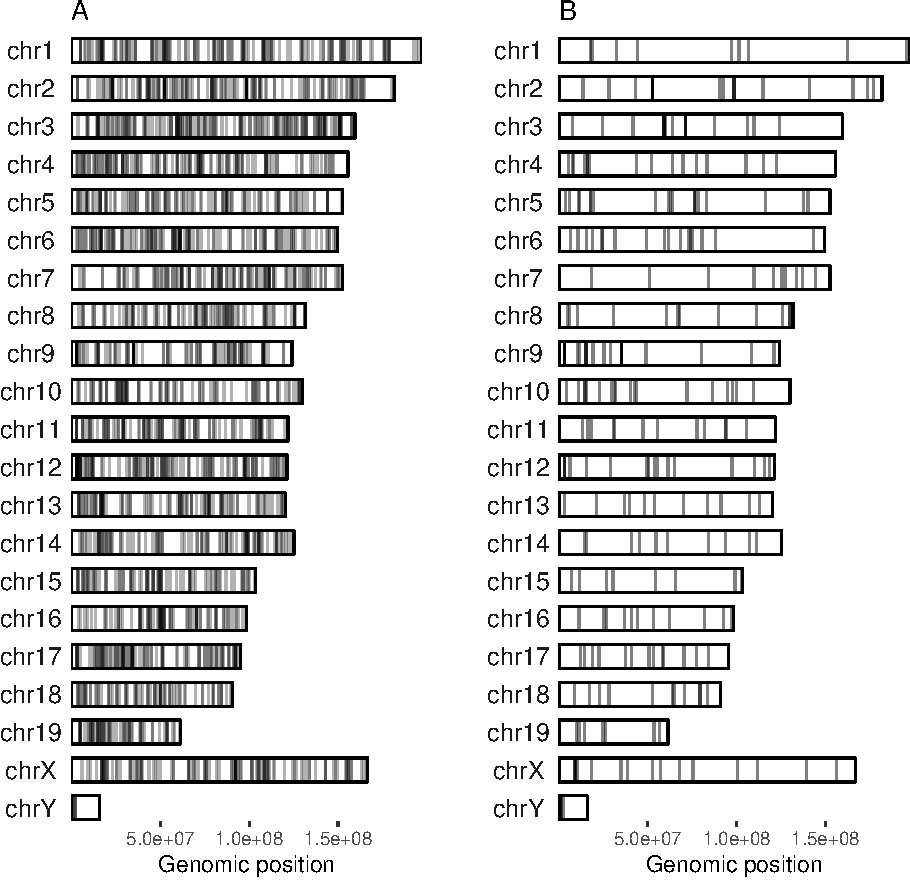
\includegraphics{project_files/figure-latex/transplantSites-1.pdf}

\newpage

Figure 6a.

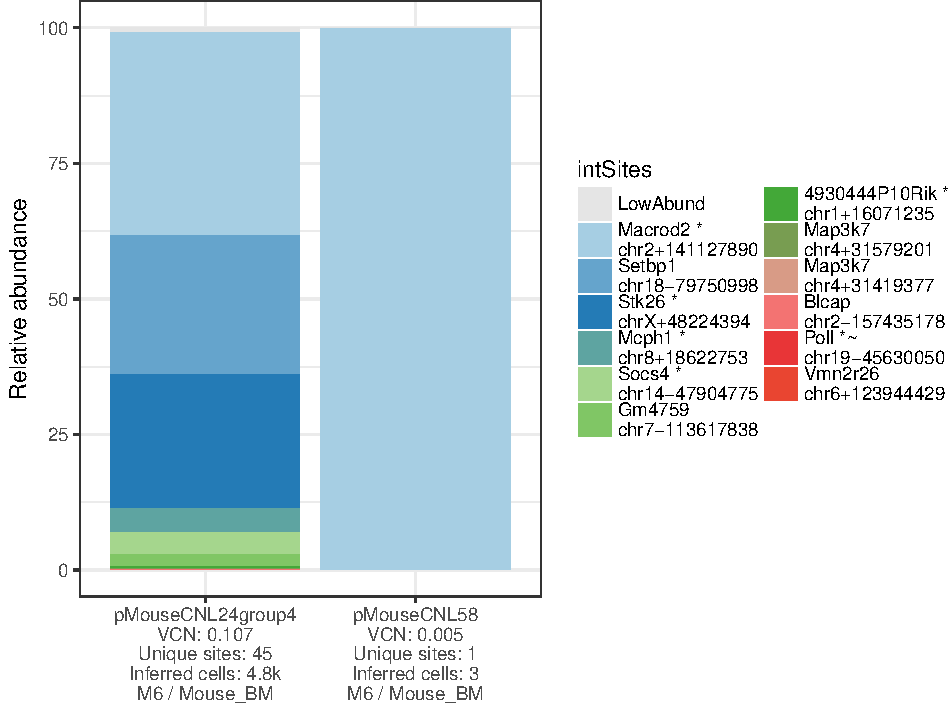
\includegraphics{project_files/figure-latex/unnamed-chunk-3-1.pdf}
\vspace{1.0cm}

\begin{table}[!h]

\caption{\label{tab:unnamed-chunk-3}Sites near oncogenes, Fisher's exact p-value: 1.000}
\centering
\begin{tabular}[t]{lrr}
\toprule
  & Not near onco & Near onco\\
\midrule
pMouseCNL24group4 & 42 & 3\\
pMouseCNL58 & 1 & 0\\
\bottomrule
\end{tabular}
\end{table}

\newpage

Figure 6b.

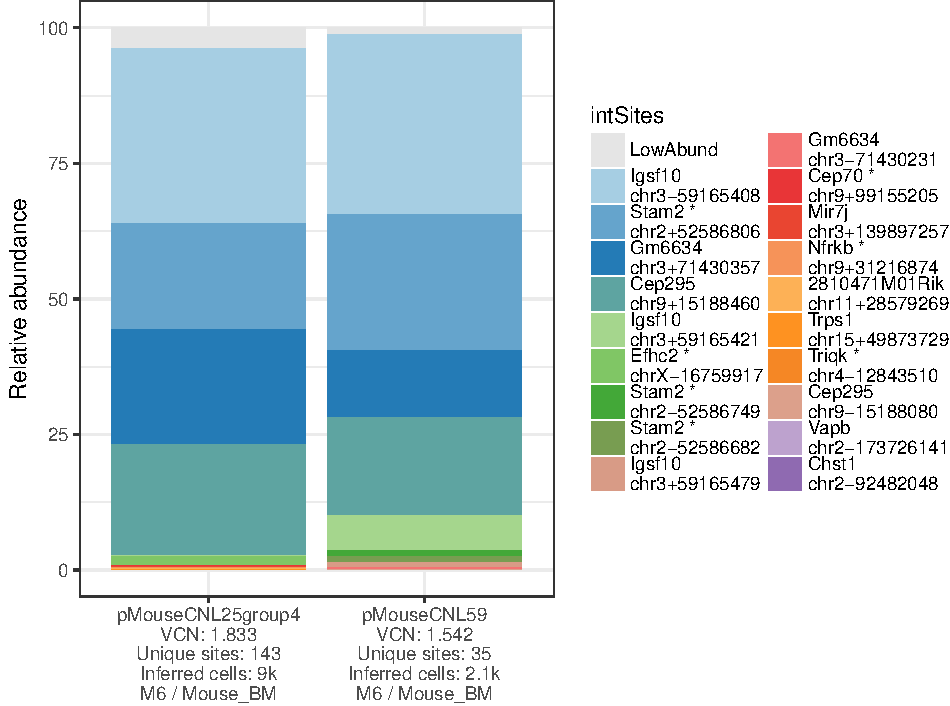
\includegraphics{project_files/figure-latex/unnamed-chunk-3-2.pdf}
\vspace{1.0cm}

\begin{table}[!h]

\caption{\label{tab:unnamed-chunk-3}Sites near oncogenes, Fisher's exact p-value: 0.208}
\centering
\begin{tabular}[t]{lrr}
\toprule
  & Not near onco & Near onco\\
\midrule
pMouseCNL25group4 & 134 & 9\\
pMouseCNL59 & 35 & 0\\
\bottomrule
\end{tabular}
\end{table}

\newpage

Figure 6c.

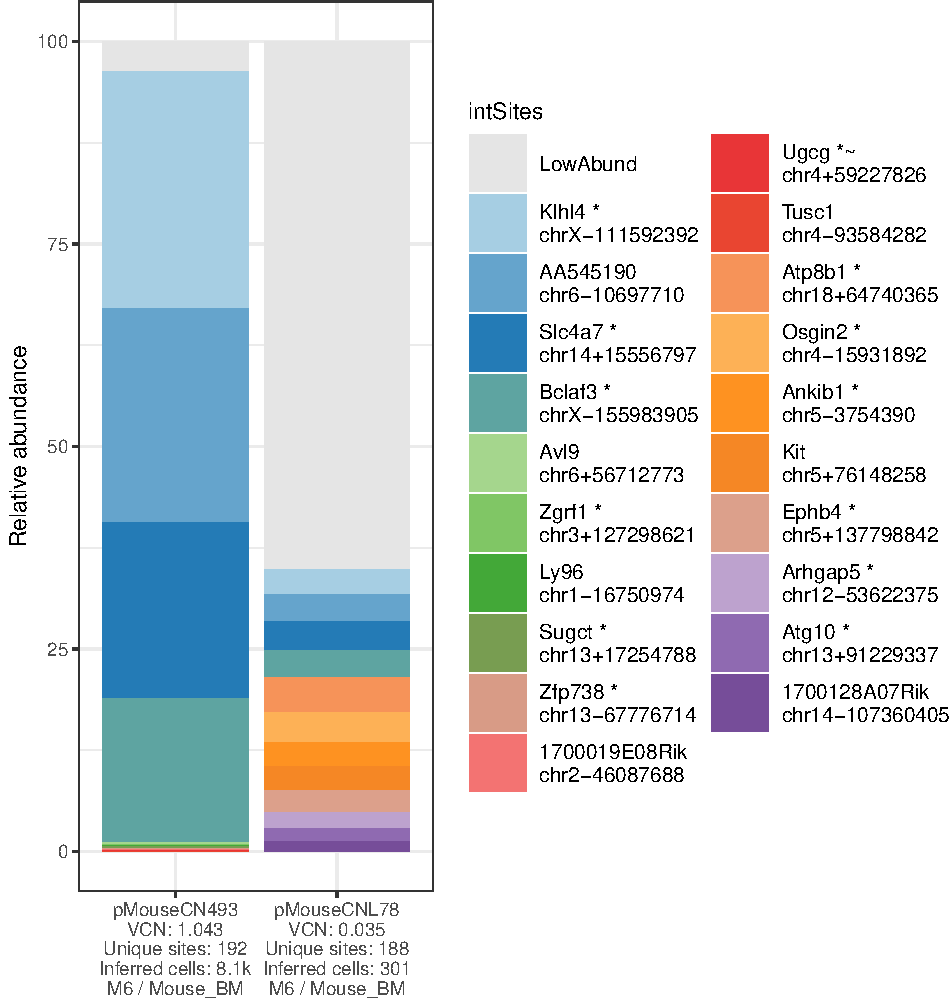
\includegraphics{project_files/figure-latex/unnamed-chunk-3-3.pdf}
\vspace{1.0cm}

\begin{table}[!h]

\caption{\label{tab:unnamed-chunk-3}Sites near oncogenes, Fisher's exact p-value: 0.647}
\centering
\begin{tabular}[t]{lrr}
\toprule
  & Not near onco & Near onco\\
\midrule
pMouseCN493 & 179 & 12\\
pMouseCNL78 & 159 & 8\\
\bottomrule
\end{tabular}
\end{table}

\newpage

Figure 6d.

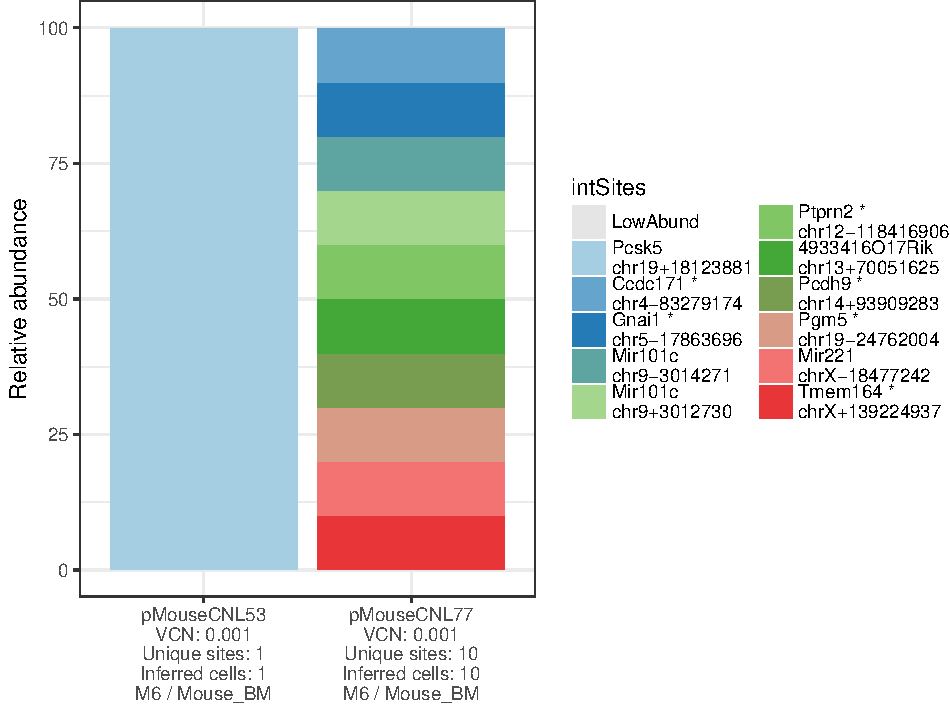
\includegraphics{project_files/figure-latex/unnamed-chunk-3-4.pdf}
\vspace{1.0cm}

\begin{table}[!h]

\caption{\label{tab:unnamed-chunk-3}Sites near oncogenes, Fisher's exact p-value: 1.000}
\centering
\begin{tabular}[t]{lrr}
\toprule
  & Not near onco & Near onco\\
\midrule
pMouseCNL53 & 1 & 0\\
pMouseCNL77 & 10 & 0\\
\bottomrule
\end{tabular}
\end{table}

\newpage

Figure 6e.

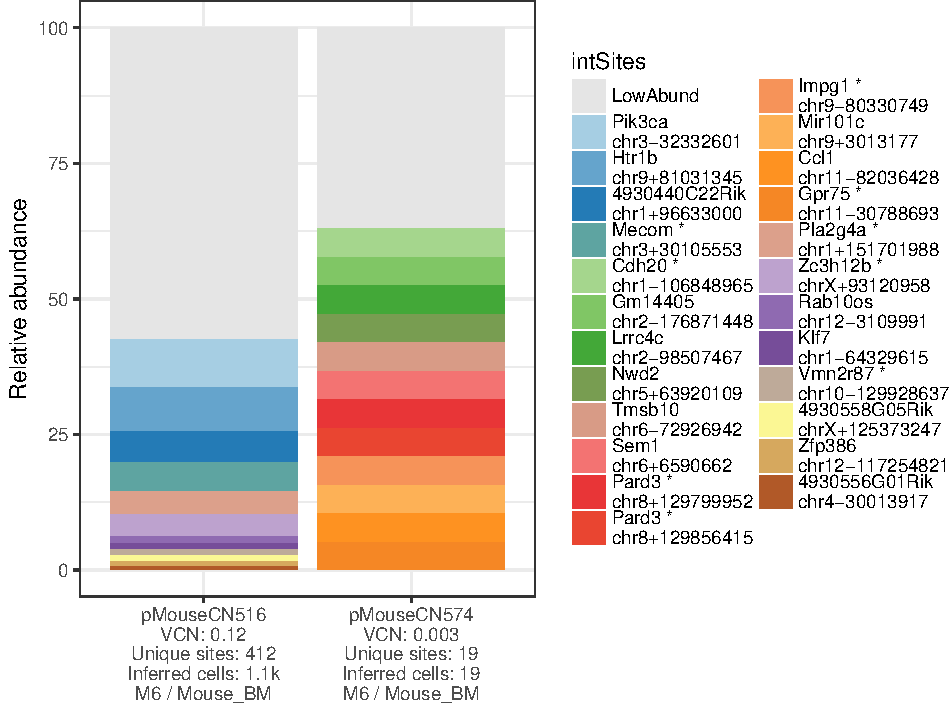
\includegraphics{project_files/figure-latex/unnamed-chunk-3-5.pdf}
\vspace{1.0cm}

\begin{table}[!h]

\caption{\label{tab:unnamed-chunk-3}Sites near oncogenes, Fisher's exact p-value: 1.000}
\centering
\begin{tabular}[t]{lrr}
\toprule
  & Not near onco & Near onco\\
\midrule
pMouseCN516 & 392 & 8\\
pMouseCN574 & 18 & 0\\
\bottomrule
\end{tabular}
\end{table}

\newpage

Figure 6f.

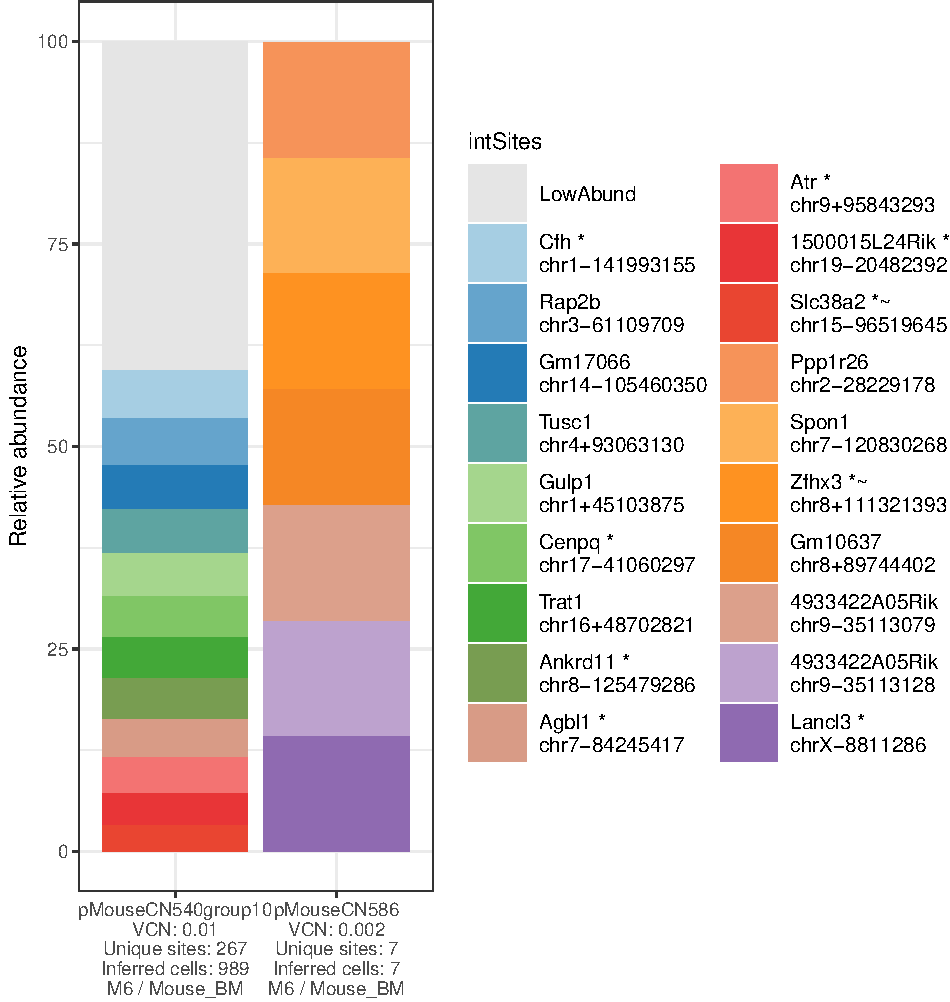
\includegraphics{project_files/figure-latex/unnamed-chunk-3-6.pdf}
\vspace{1.0cm}

\begin{table}[!h]

\caption{\label{tab:unnamed-chunk-3}Sites near oncogenes, Fisher's exact p-value: 0.415}
\centering
\begin{tabular}[t]{lrr}
\toprule
  & Not near onco & Near onco\\
\midrule
pMouseCN540group10 & 248 & 19\\
pMouseCN586 & 6 & 1\\
\bottomrule
\end{tabular}
\end{table}

\newpage

Figure 6g.

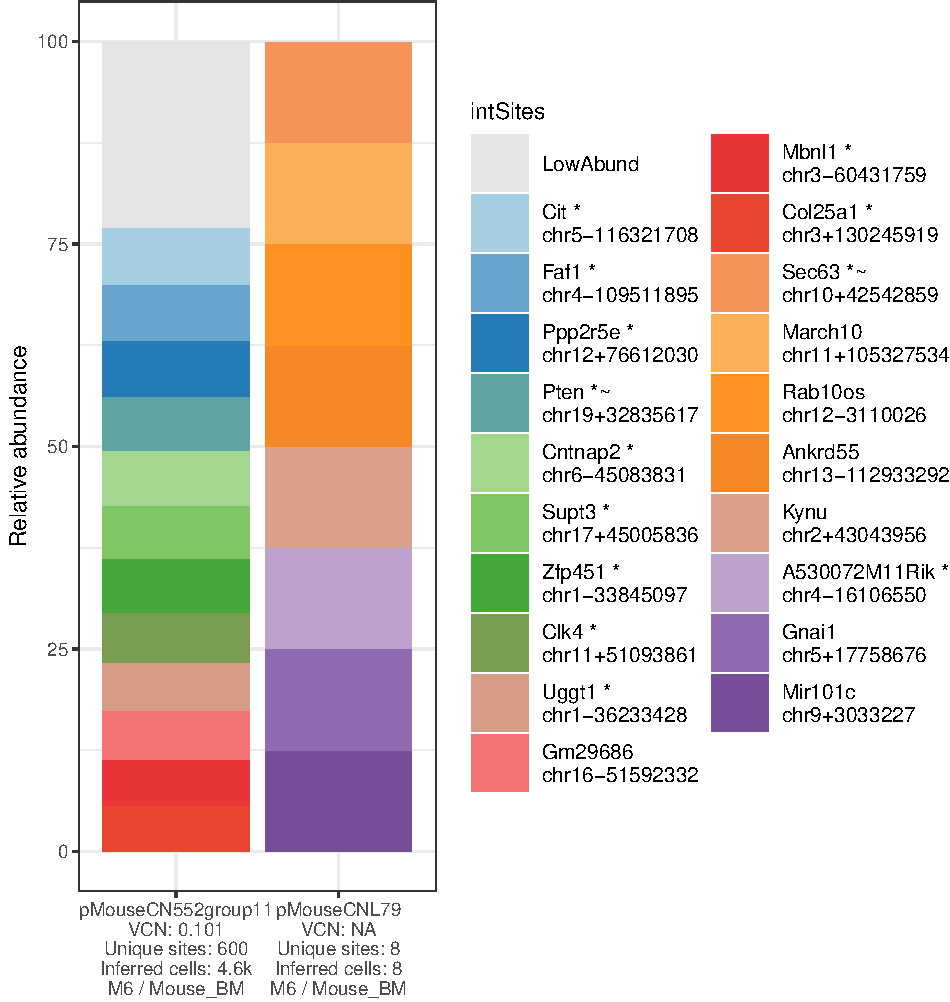
\includegraphics{project_files/figure-latex/unnamed-chunk-3-7.pdf}
\vspace{1.0cm}

\begin{table}[!h]

\caption{\label{tab:unnamed-chunk-3}Sites near oncogenes, Fisher's exact p-value: 0.366}
\centering
\begin{tabular}[t]{lrr}
\toprule
  & Not near onco & Near onco\\
\midrule
pMouseCN552group11 & 559 & 32\\
pMouseCNL79 & 7 & 1\\
\bottomrule
\end{tabular}
\end{table}

\newpage

Figure 6h.

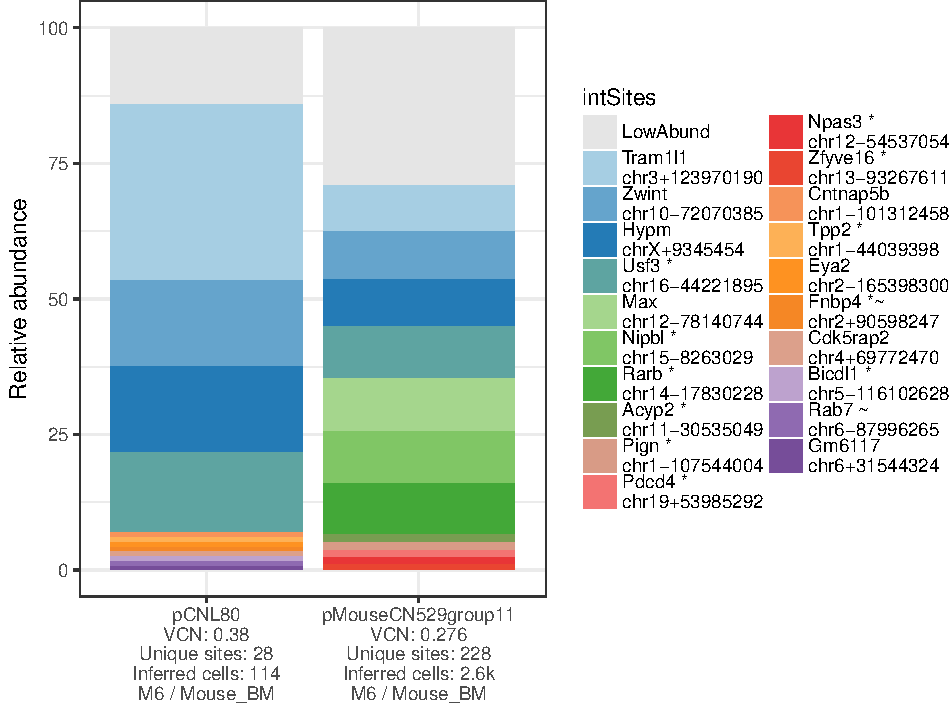
\includegraphics{project_files/figure-latex/unnamed-chunk-3-8.pdf}
\vspace{1.0cm}

\begin{table}[!h]

\caption{\label{tab:unnamed-chunk-3}Sites near oncogenes, Fisher's exact p-value: 0.673}
\centering
\begin{tabular}[t]{lrr}
\toprule
  & Not near onco & Near onco\\
\midrule
pMouseCN529group11 & 214 & 13\\
pCNL80 & 26 & 2\\
\bottomrule
\end{tabular}
\end{table}

\newpage

Figure 6i.

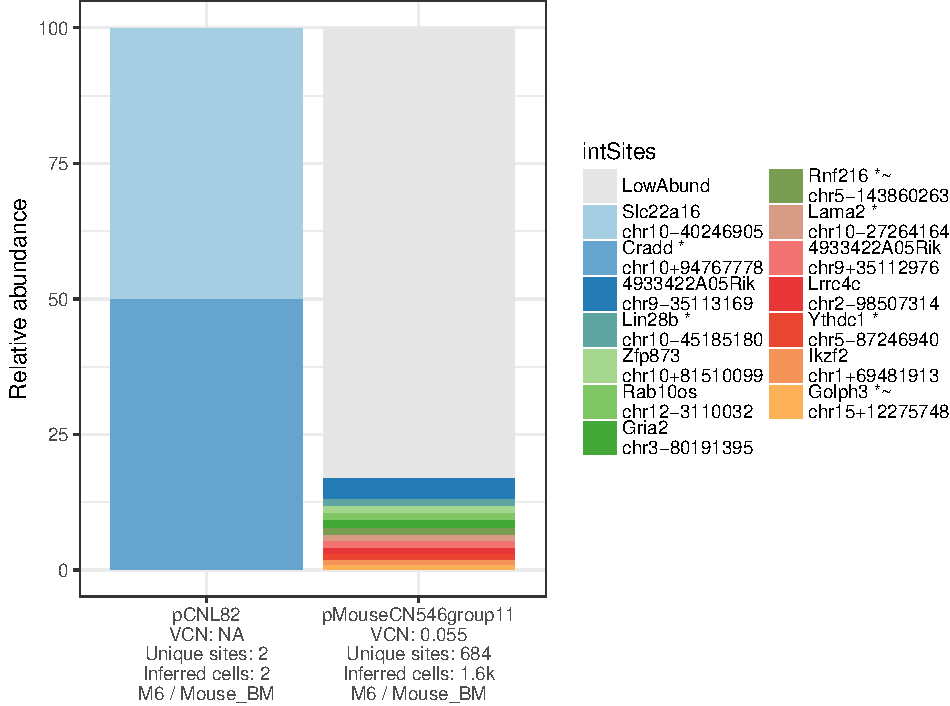
\includegraphics{project_files/figure-latex/unnamed-chunk-3-9.pdf}
\vspace{1.0cm}

\begin{table}[!h]

\caption{\label{tab:unnamed-chunk-3}Sites near oncogenes, Fisher's exact p-value: 1.000}
\centering
\begin{tabular}[t]{lrr}
\toprule
  & Not near onco & Near onco\\
\midrule
pMouseCN546group11 & 646 & 25\\
pCNL82 & 2 & 0\\
\bottomrule
\end{tabular}
\end{table}

\newpage

\newpage

\textbf{Analyst}


\includegraphics[width=4.04in]{./data/Everett_signature}

John K. Everett, Ph.D.

\vspace{0.5cm}

\textbf{Laboratory director}

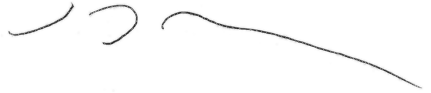
\includegraphics[width=5.99in]{./data/Bushman_signature}

Frederic D. Bushman, Ph.D.

\vspace{2.0cm}

\section{References}\label{references}

\begin{enumerate}
\def\labelenumi{\arabic{enumi}.}
\tightlist
\item
  RTCGD: retroviral tagged cancer gene database. Akagi K, Suzuki T,
  Stephens RM, Jenkins NA, Copeland NG. Nucleic Acids Res. 2004 Jan
  1;32(Database issue):D523-7.
\end{enumerate}

\vspace{0.1cm}

\begin{enumerate}
\def\labelenumi{\arabic{enumi}.}
\setcounter{enumi}{1}
\tightlist
\item
  Outcomes following gene therapy in patients with severe
  Wiskott-Aldrich syndrome. Hacein-Bey Abina S, Gaspar HB, Blondeau J,
  Caccavelli L, Charrier S, Buckland K, Picard C, Six E, Himoudi N,
  Gilmour K, McNicol AM, Hara H, Xu-Bayford J, Rivat C, Touzot F,
  Mavilio F, Lim A, Treluyer JM, Héritier S, Lefrère F, Magalon J,
  Pengue-Koyi I, Honnet G, Blanche S, Sherman EA, Male F, Berry C,
  Malani N, Bushman FD, Fischer A, Thrasher AJ, Galy A, Cavazzana M.
  JAMA. 2015 Apr 21;313(15):1550-63.
\end{enumerate}

\vspace{0.1cm}

\begin{enumerate}
\def\labelenumi{\arabic{enumi}.}
\setcounter{enumi}{2}
\tightlist
\item
  Distribution of Lentiviral Vector Integration Sites in Mice Following
  Therapeutic Gene Transfer to Treat \(\beta\)-thalassemia. Ronen K,
  Negre O, Roth S, Colomb C, Malani N, Denaro M, Brady T, Fusil F,
  Gillet-Legrand B, Hehir K, Beuzard Y, Leboulch P, Down JD, Payen E,
  Bushman FD. Mol Ther. 2011 Jul;19(7):1273-86.
\end{enumerate}

\vspace{0.1cm}

\begin{enumerate}
\def\labelenumi{\arabic{enumi}.}
\setcounter{enumi}{3}
\tightlist
\item
  Estimating abundances of retroviral insertion sites from DNA fragment
  length data. Berry CC, Gillet NA, Melamed A, Gormley N, Bangham CR,
  Bushman FD. Bioinformatics. 2012 Mar 15;28(6):755-62.
\end{enumerate}

\vspace{0.1cm}

\begin{enumerate}
\def\labelenumi{\arabic{enumi}.}
\setcounter{enumi}{4}
\tightlist
\item
  INSPIIRED: A Pipeline for Quantitative Analysis of Sites of New DNA
  Integration in Cellular Genomes. Sherman E, Nobles C, Berry CC, Six E,
  Wu Y, Dryga A, Malani N, Male F, Reddy S, Bailey A, Bittinger K,
  Everett JK, Caccavelli L, Drake MJ, Bates P, Hacein-Bey-Abina S,
  Cavazzana M, Bushman FD. Mol Ther Methods Clin Dev. 2016 Dec
  18;4:39-49.
\end{enumerate}

\newpage

\section{Supplementary tables and
figures}\label{supplementary-tables-and-figures}

\subsection{Numbers of inferred cells and integration sites identified
in provided
samples}\label{numbers-of-inferred-cells-and-integration-sites-identified-in-provided-samples}

\emph{Table S1.}\\

\begin{table}[H]
\centering\rowcolors{2}{gray!6}{white}

\resizebox{\linewidth}{!}{\begin{tabular}{llllrlll}
\hiderowcolors
\toprule
organism & GTSP & Subject & Cell type & VCN & Time point & Number inferred cells & Number of intSites\\
\midrule
\showrowcolors
human & GTSP0689 & pCYS002NS & PBCD34-MOI20 & 0.940 & D14 & 2,978 & 1,468\\
human & GTSP0691 & pCYS004BR & PBCD34-MOI20 & 0.930 & D14 & 1,034 & 764\\
human & GTSP0692 & pCYS005OB & PB\_CD34 & 0.970 & D14 & 8,384 & 3,297\\
human & GTSP1369 & pDON.002.4.SC & PB\_CD34 & 4.520 & D14 & 127 & 44\\
human & GTSP1370 & pDON.003.2.SG & PB\_CD34 & 2.440 & D14 & 1,482 & 1,188\\
human & GTSP1371 & pDON.007.CR & PB\_CD34 & 1.270 & D14 & 122 & 86\\
human & GTSP1372 & pDON.008.LH & PB\_CD34 & 2.530 & D14 & 124 & 100\\
human & GTSP1373 & pDON.009.JH & PB\_CD34 & 5.280 & D14 & 757 & 606\\
human & GTSP1374 & pDON.010.CC & PB\_CD34 & 3.290 & D14 & 513 & 371\\
human & GTSP1375 & pCYS.013.PS & PBCD34-mock & NA & D14 & 1 & 1\\
human & GTSP1376 & pCYS.007.2.BS & PBCD34-mock & 0.002 & D14 & 4 & 4\\
human & GTSP1377 & pCYS.002.4.NS & PB\_CD34 & 2.400 & D14 & 102 & 54\\
human & GTSP1378 & pCYS.007.2.BS & PBCD34-MOI20 & 3.640 & D14 & 543 & 462\\
human & GTSP1379 & pCYS.007.2.BS & PBCD34-MOI40 & 6.100 & D14 & 1,210 & 1,060\\
human & GTSP1380 & pCYS.013.PS & PBCD34-MOI40 & 1.000 & D14 & 44 & 25\\
human & GTSP1682 & pCYS\_017\_BW\_MOI2x107 & PB\_CD34 & 1.660 & D14 & 16,696 & 11,689\\
human & GTSP1683 & pCYS\_017\_BW\_MOI6x106 & PB\_CD34 & 1.415 & D14 & 16,690 & 11,090\\
human & GTSP1685 & pCYS\_018\_MM\_MOI2x107 & PB\_CD34 & 0.958 & D14 & 11,679 & 8,444\\
human & GTSP1686 & pCYS\_018\_MM\_MOI6x106 & PB\_CD34 & 0.530 & D14 & 7,089 & 4,547\\
human & GTSP1687 & pCYS\_018\_MM\_MOI2x106 & PB\_CD34 & 0.331 & D14 & 3,594 & 2,508\\
human & GTSP1688 & pCYS\_020\_JJ & PB\_CD34 & 2.590 & D14 & 21,709 & 14,755\\
human & GTSP1689 & pMP011.1.Ch2 & PB\_CD34 & 1.607 & D14 & 1,500 & 940\\
human & GTSP1690 & pSC002.6.Ch7 & PB\_CD34 & 2.350 & D14 & 401 & 222\\
human & GTSP1691 & pMP011.1.Ch9 & PB\_CD34 & 2.420 & D14 & 692 & 427\\
human & GTSP1692 & pMP011.1.Ch11 & PB\_CD34 & 1.074 & D14 & 596 & 353\\
human & GTSP1694 & pDON.004.3.TL.MOI20 & PB\_CD34 & 3.250 & D14 & 5,273 & 4,569\\
human & GTSP1695 & pDON.011.2.MP & PB\_CD34 & 3.950 & D14 & 11,199 & 7,065\\
human & GTSP1969 & pLSR1TEST2 & BM CD34+ Cells & 0.695 & 0 & 2,568 & 2,215\\
human & GTSP1970 & pLSR1THAW2 & BM CD34+ Cells & 0.709 & 0 & 6,320 & 6,009\\
human & GTSP1971 & pLSR2Thaw2 & BM CD34+ Cells & 1.020 & 0 & 9,188 & 8,687\\
\bottomrule
\end{tabular}}
\rowcolors{2}{white}{white}
\end{table}

\newpage

\emph{Table S1 (continued).}\\

\begin{table}[H]
\centering\rowcolors{2}{gray!6}{white}

\resizebox{\linewidth}{!}{\begin{tabular}{llllrlll}
\hiderowcolors
\toprule
organism & GTSP & Subject & Cell type & VCN & Time point & Number inferred cells & Number of intSites\\
\midrule
\showrowcolors
mouse & GTSP0829 & pMouseCNL23group4control & Mouse\_BM & NA & M6 & 6 & 5\\
mouse & GTSP0830 & pMouseCNL24group4 & Mouse\_BM & 0.107 & M6 & 4,797 & 45\\
mouse & GTSP0831 & pMouseCNL25group4 & Mouse\_BM & 1.833 & M6 & 9,000 & 143\\
mouse & GTSP0832 & pMouseCNL38group1A & Mouse\_BM & NA & M6 & 2 & 2\\
mouse & GTSP0833 & pMouseCulture & Mouse\_Sca1pos & 2.760 & D14 & 80 & 28\\
mouse & GTSP0891 & pMouseCN493 & Mouse\_BM & 1.043 & M6 & 8,143 & 192\\
mouse & GTSP0892 & pMouseCNL53 & Mouse\_BM & 0.001 & M6 & 1 & 1\\
mouse & GTSP0947 & pMouseCNL58 & Mouse\_BM & 0.005 & M6 & 3 & 1\\
mouse & GTSP0948 & pMouseCNL59 & Mouse\_BM & 1.542 & M6 & 2,087 & 35\\
mouse & GTSP0949 & pMouseCN516 & Mouse\_BM & 0.120 & M6 & 1,108 & 412\\
mouse & GTSP0950 & pMouseCN518 & Mouse\_BM & 2.430 & M6 & 3,399 & 103\\
mouse & GTSP1079 & pMouseCN540group10 & Mouse\_BM & 0.010 & M6 & 989 & 267\\
mouse & GTSP1080 & pMouseCN552group11 & Mouse\_BM & 0.101 & M6 & 4,636 & 602\\
mouse & GTSP1081 & pMouseCN529group11 & Mouse\_BM & 0.276 & M6 & 2,610 & 228\\
mouse & GTSP1082 & pMouseCN545group11 & Mouse\_BM & 1.798 & M6 & 5,268 & 35\\
mouse & GTSP1083 & pMouseCN546group11 & Mouse\_BM & 0.055 & M6 & 1,603 & 684\\
mouse & GTSP1084 & pMouseCNL70group12 & Mouse\_BM & NA & M6 & 1,121 & 94\\
mouse & GTSP1146 & pMouseCN557 & Mouse\_BM & 1.597 & M6 & 14,244 & 745\\
mouse & GTSP1147 & pMouseCNL77 & Mouse\_BM & 0.001 & M6 & 10 & 10\\
mouse & GTSP1148 & pMouseCNL78 & Mouse\_BM & 0.035 & M6 & 301 & 188\\
mouse & GTSP1149 & pMouseCN574 & Mouse\_BM & 0.003 & M6 & 19 & 19\\
mouse & GTSP1150 & pMouseCN586 & Mouse\_BM & 0.002 & M6 & 7 & 7\\
mouse & GTSP1151 & pMouseCNL79 & Mouse\_BM & NA & M6 & 8 & 8\\
mouse & GTSP1481 & pCNL80 & Mouse\_BM & 0.380 & M6 & 114 & 28\\
mouse & GTSP1482 & pCNL82 & Mouse\_BM & NA & M6 & 2 & 2\\
mouse & GTSP1696 & pCN665 & Mouse\_BM & 4.490 & M6 & 3,706 & 190\\
mouse & GTSP1697 & pCN671 & Mouse\_BM & 0.486 & M6 & 5,515 & 247\\
mouse & GTSP1705 & pCN552 & Bone Marrow & NA & M6 & 63 & 15\\
mouse & GTSP1706 & pCN552 & T-Cells & NA & M6 & 174 & 49\\
mouse & GTSP1707 & pCN552 & B Cells & NA & M6 & 865 & 161\\
mouse & GTSP1708 & pCN552 & Bone Marrow & NA & M6 & 467 & 104\\
mouse & GTSP1709 & pCNL59 & Bone Marrow & NA & M6 & 88 & 6\\
mouse & GTSP1710 & pCNL59 & Bone Marrow & NA & M6 & 68 & 5\\
mouse & GTSP1712 & pCNL59 & B Cells & NA & M6 & 18 & 4\\
mouse & GTSP1867 & pCN746 & Bone Marrow & NA & M6 & 141 & 34\\
mouse & GTSP1972 & pCN752 & Bone Marrow & 0.004 & 6M & 225 & 74\\
mouse & GTSP1973 & pCN755 & Bone Marrow & NA & 6M & 28 & 27\\
mouse & GTSP1974 & pCN760 & Bone Marrow & 0.001 & 6M & 16 & 10\\
mouse & GTSP1977 & pCN774 & Bone Marrow & 0.039 & 6M & 448 & 191\\
mouse & GTSP1978 & pCN801 & Bone Marrow & 10.490 & 6M & 15,278 & 102\\
mouse & GTSP1979 & pCN803 & Bone Marrow & 0.654 & 6M & 2,254 & 149\\
mouse & GTSP1980 & pCN804 & Bone Marrow & 0.003 & 6M & 68 & 28\\
mouse & GTSP1981 & pCN806 & Bone Marrow & 0.001 & 6M & 8 & 8\\
mouse & GTSP1982 & pCN809 & Bone Marrow & 0.572 & 6M & 2,588 & 101\\
\bottomrule
\end{tabular}}
\rowcolors{2}{white}{white}
\end{table}

\newpage

\subsection{Analyzed samples in which no integration sites were
identified}\label{analyzed-samples-in-which-no-integration-sites-were-identified}

\emph{Table S2.}\\

\begin{table}[H]
\centering\rowcolors{2}{gray!6}{white}

\resizebox{\linewidth}{!}{\begin{tabular}{lllll}
\hiderowcolors
\toprule
SpecimenAccNum & CellType & Patient & Timepoint & SpecimenInfo\\
\midrule
\showrowcolors
GTSP0688 & PBCD34-mock & pCYS002NS & d14 & Mock transduced control; Stage: Mock\\
GTSP0690 & PBCD34-mock & pCYS004BR & d14 & Mock transduced control; Stage: Mock\\
GTSP0828 & Mouse\_BM & pMouseCNL1group1 & m6 & pCCL-CTNS; MOI 10; Stage: Primary\\
GTSP0834 & Mouse\_Sca1pos & pMouseCultureControl & d14 & Control, DNA was extracted from mouse Sca1+ cells and cultured for 2 weeks (Mock); Stage:\\
GTSP1684 & PB\_CD34 & pCYS\_017\_BW\_MOCK & d14 & Mock transduced control; Stage: Mock\\
GTSP1693 & PB\_CD34 & pDON.004.3.TL.MOCK & d14 & Mock transduced control; Stage: Mock\\
GTSP1711 & T-Cells & pCNL59 & m6 & Mouse Thymus, T cells\\
GTSP1868 & Bone Marrow & pCN748 & m6 & "pCCL-CTNS transduced, Secondary graft, Primary graft mouse: CN671, Primary graft VCN: 1.31"\\
GTSP1975 & DNA & pCN752P1 & 6m & "Mouse, ""growth"" P=pathology sample 1 from CN752 (found in thorax) labelled ""Growth"""\\
GTSP1976 & DNA & pCN752P2 & 6m & Mouse P=pathology sample 2 from CN752(thymus)\\
\bottomrule
\end{tabular}}
\rowcolors{2}{white}{white}
\end{table}

\newpage

\subsection{Comparison of the number of integration sites and inferred
cells}\label{comparison-of-the-number-of-integration-sites-and-inferred-cells}

Kolmogorov--Smirnov tests show no significant differences between the
distributions of estimated abundances between trials. The plot below was
truncated at 100 inferred cells for clarity which eliminated 16 data
points from the `WAS m12' distriubtion.

\emph{Figure S1.}

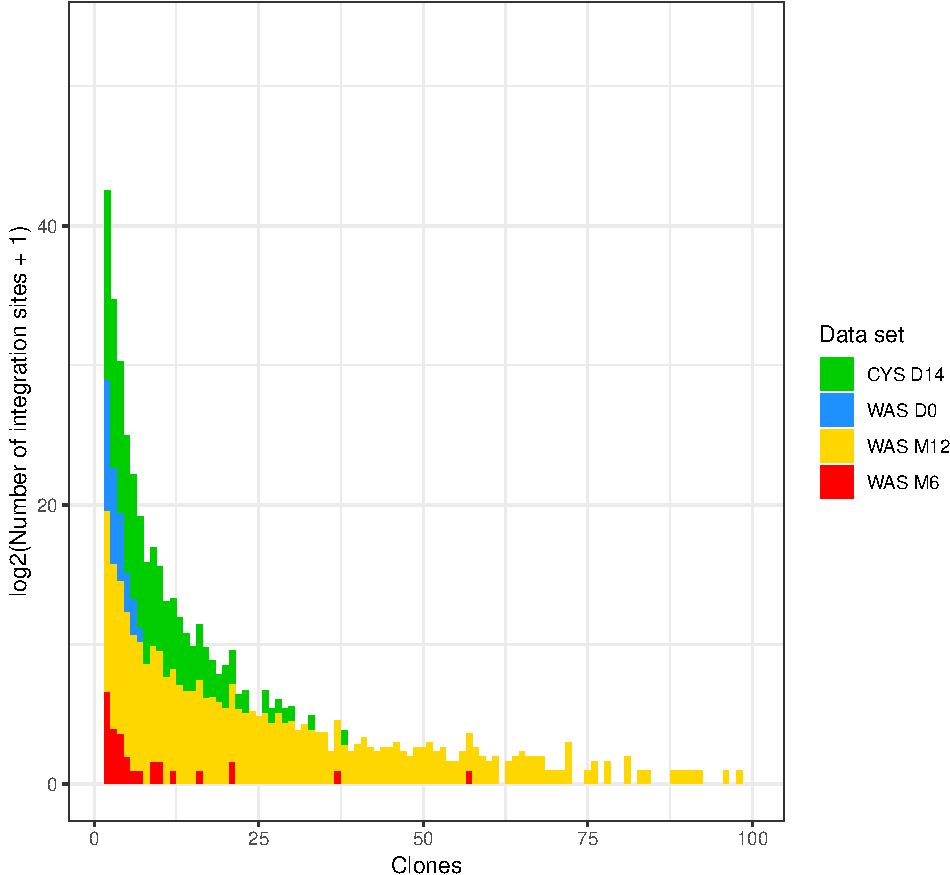
\includegraphics{project_files/figure-latex/FigS1-1.pdf}

\newpage

\subsection{\texorpdfstring{Integration positions of the lentiviral
theraputic vector from a previous WAS correction
trial\textsuperscript{1}}{Integration positions of the lentiviral theraputic vector from a previous WAS correction trial1}}\label{integration-positions-of-the-lentiviral-theraputic-vector-from-a-previous-was-correction-trial1}

\emph{Figure S2.}

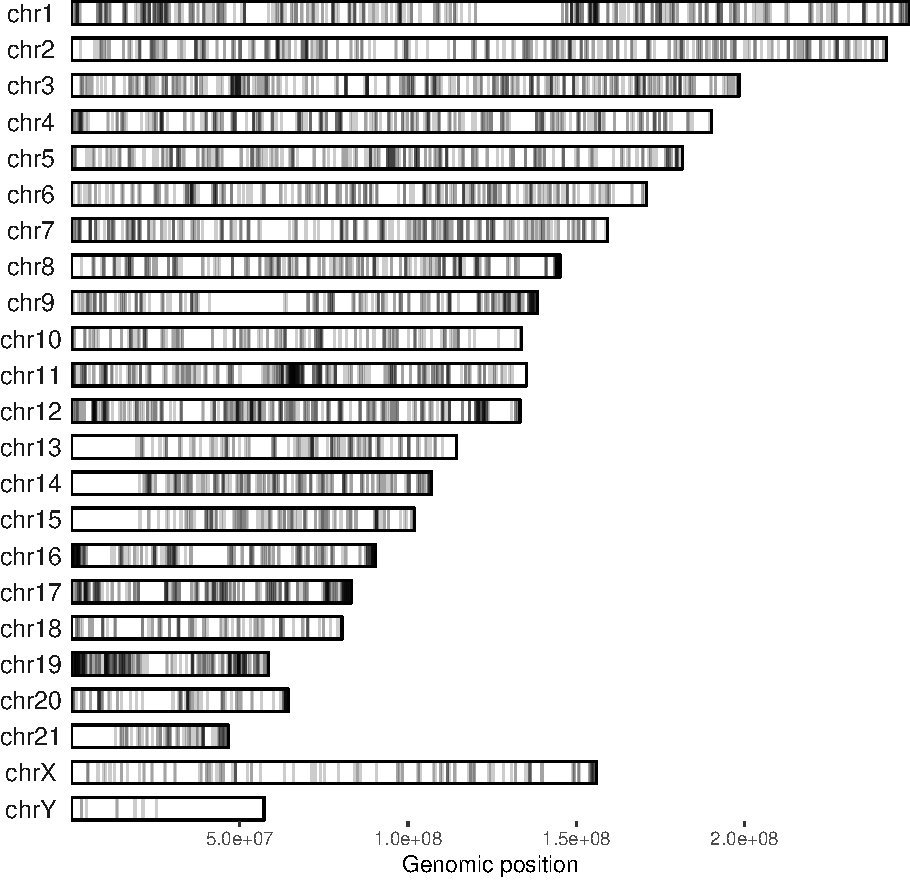
\includegraphics{project_files/figure-latex/FigS2-1.pdf}

\newpage

\subsection{Persistence of clones in mouse BM transplant
trials}\label{persistence-of-clones-in-mouse-bm-transplant-trials}

\emph{Table S3.}

\begin{table}[H]
\centering\rowcolors{2}{gray!6}{white}

\resizebox{\linewidth}{!}{\begin{tabular}{lllll}
\hiderowcolors
\toprule
Donor & Recipient & intSite & Donor cells & Recipient cells\\
\midrule
\showrowcolors
pMouseCNL24group4 & pMouseCNL58 & chr2+141127890 & 1,796 & 3\\
pMouseCNL25group4 & pMouseCNL59 & chr2-52586749 & 7 & 25\\
pMouseCNL25group4 & pMouseCNL59 & chr2-52586682 & 1 & 23\\
pMouseCNL25group4 & pMouseCNL59 & chr2+52586806 & 1,764 & 525\\
pMouseCNL25group4 & pMouseCNL59 & chr3-71430231 & 2 & 8\\
pMouseCNL25group4 & pMouseCNL59 & chr3-59165408 & 2,907 & 690\\
pMouseCNL25group4 & pMouseCNL59 & chr3+59165404 & 1 & 1\\
pMouseCNL25group4 & pMouseCNL59 & chr3+59165421 & 26 & 134\\
pMouseCNL25group4 & pMouseCNL59 & chr3+59165479 & 6 & 19\\
pMouseCNL25group4 & pMouseCNL59 & chr3+71430357 & 1,907 & 260\\
pMouseCNL25group4 & pMouseCNL59 & chr9+15188460 & 1,838 & 375\\
pMouseCNL25group4 & pMouseCNL59 & chr12-55631198 & 3 & 1\\
pMouseCN493 & pMouseCNL78 & chr6-10697710 & 2,161 & 10\\
pMouseCN493 & pMouseCNL78 & chr14+15556797 & 1,769 & 11\\
pMouseCN493 & pMouseCNL78 & chrX-155983905 & 1,445 & 10\\
pMouseCN493 & pMouseCNL78 & chrX-111592392 & 2,375 & 9\\
pMouseCN540group10 & pMouseCN586 & chr9-35113079 & 1 & 1\\
pMouseCN552group11 & pMouseCNL79 & chr12-3110022 & 10 & 1\\
pMouseCN529group11 & pCNL80 & chr3+123970190 & 221 & 37\\
pMouseCN529group11 & pCNL80 & chr10-72070385 & 235 & 18\\
pMouseCN529group11 & pCNL80 & chr16-44221895 & 246 & 17\\
pMouseCN529group11 & pCNL80 & chrX+9345454 & 226 & 18\\
\bottomrule
\end{tabular}}
\rowcolors{2}{white}{white}
\end{table}

\newpage

\subsection{Sequencing depth}\label{sequencing-depth}

Identified integration site are shown as colored squares that are
positioned by the number of reads leading to their identification.

\emph{Figure S3.}

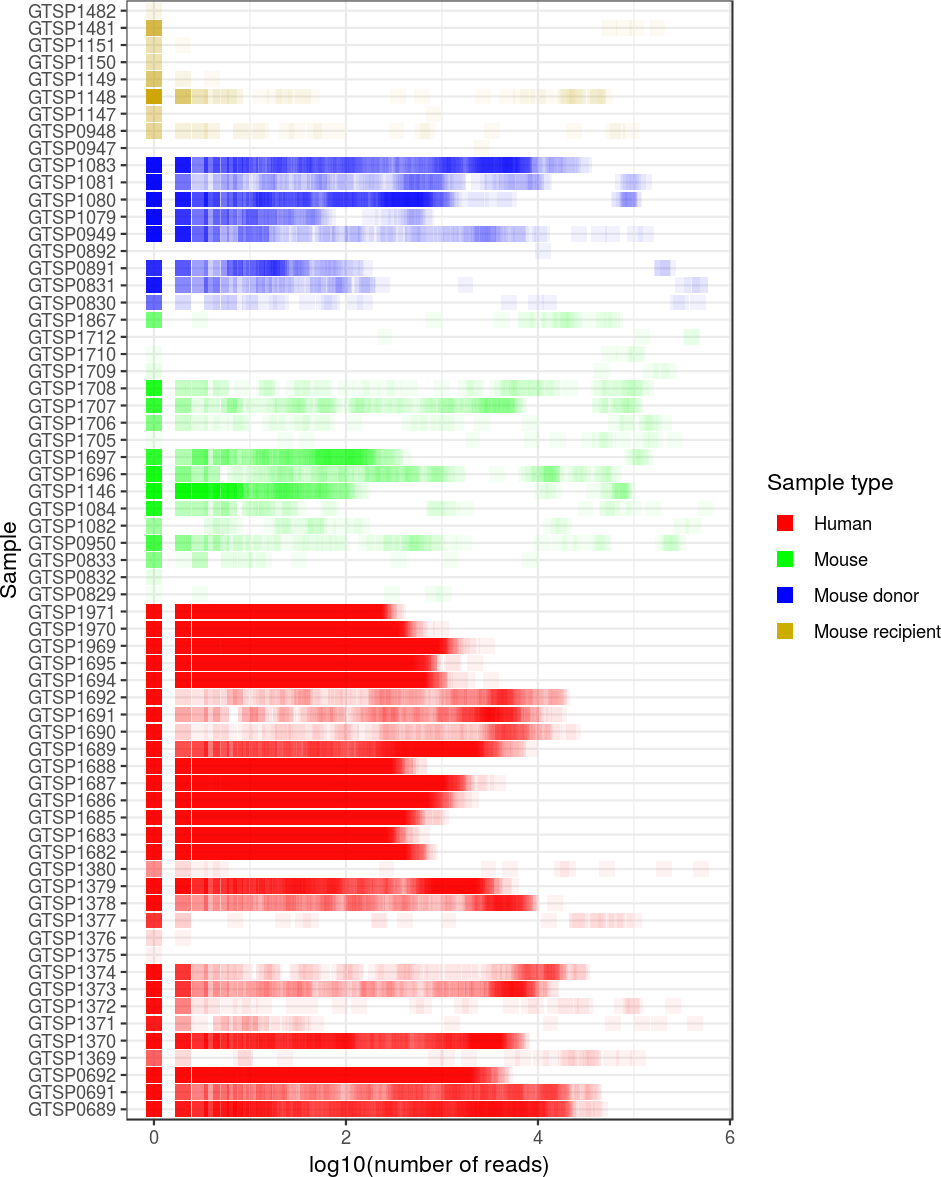
\includegraphics{project_files/figure-latex/FigS3-1.png}


\end{document}
